\begin{itemize}
    \item Análisis del problema
        \begin{itemize}
        
            \item Descripción general:
            El sistema de riego automático para cultivo de tomate monitorea continuamente la humedad relativa del ambiente mediante un sensor digital DHT11. Cuando la humedad desciende por debajo de un umbral mínimo, activa una bomba de agua (mediante relé) para iniciar el riego. El proceso se detiene al alcanzar el nivel de humedad óptimo. Se implementa histéresis para evitar ciclos de encendido/apagado rápidos y temporización no bloqueante para garantizar un funcionamiento secuencial estable. La información del sistema se visualiza en una pantalla OLED I2C de 0.96".

        \end{itemize} 

        \item Identificación de Entradas y Salidas
        \begin{itemize}
            
            \item Entradas:
                \begin{itemize}
                    \item  Sensor DHT11: señal digital en pin D2 (humedad relativa y temperatura).

                    \item Botón de riego manual (override): pin digital D3.                  
                \end{itemize}
            
            \item Salidas:
                \begin{itemize}
                    \item Módulo relé 5V: activa/desactiva la bomba de agua.
                    \item LED verde: humedad adecuada (IDLE).    
                    \item LED azul/amarillo: riego activo (REGANDO).
                    \item LED rojo: humedad crítica baja (ALARMA).
                    \item Pantalla OLED I2C 0.96" 128x64: visualización del porcentaje de humedad y estado del sistema.
                \end{itemize}
        \end{itemize}

        \item Restricciones técnicas
            \begin{itemize}
                \item No se debe usar delay() en el ciclo principal.
                \item Implementación de histéresis en umbrales de humedad.
                \item El sistema debe operar de forma completamente autónoma sin intervención humana.
                \item Separación de la lógica de negocio del control de hardware.
                \item El DHT11 requiere un intervalo mínimo de 2000 ms entre lecturas.
                \item Tiempo mínimo de riego: 5 segundos para evitar micro-ciclos.
                
            \end{itemize}

        \item Definición de umbrales y variables:

        En la Tabla~\ref{tab:Table_1_R3}, se observa la definición de las variables con sus respectivas descripciones y justificación. Reconocer las variables a utilizar sera de ayuda a la hora de realizar el código.

        \begin{table}[ht]
\caption{Variables Involucradas (Sistema de Riego Automático)}
\label{tab:Table_1_R3}
\centering
\renewcommand{\arraystretch}{1.3}
\begin{tabularx}{\columnwidth}{X p{2.0cm} p{2.0cm}}
\toprule
\textbf{Variable} & \textbf{Tipo} & \textbf{Valor / Rango} \\
\midrule
UMBRAL\_SECO   & const int    & 30\%       \\
UMBRAL\_HUMEDO & const int    & 70\%       \\
UMBRAL\_ALARMA & const int    & 20\%       \\
HISTERESIS     & const int    & 5\%        \\
humedadActual  & float        & 0--100\%   \\
estadoRiego    & enum         & IDLE / REGANDO / ALARMA \\
bombaActiva    & bool         & true / false \\
tiempoInicioRiego & unsigned long & ms      \\
tiempoMinRiego & const long   & 5000 ms    \\
\midrule
\textbf{Total} & \textbf{9 variables} & --- \\
\bottomrule
\end{tabularx}
\end{table}

        \item Flujograma del Sistema

        El sistema opera mediante un ciclo continuo con lecturas periódicas del sensor DHT11 cada 2000 ms. La lógica de control de la bomba se ejecuta basándose en el estado actual y los valores de humedad medidos, aplicando histéresis para garantizar estabilidad.

        \begin{algorithm}[ht]
\caption{Algoritmo de Sistema de Riego Automático}
\label{alg:Algoritmo_Riego}
\begin{algorithmic}[1]
\Statex \textbf{Inicialización:}
\State Inicializar pines, YI69, relé en OFF y pantalla OLED
\State $estadoRiego = IDLE$
\State $bombaActiva = false$
\While{true}
    \If{$millis() - tiempoUltimaLectura \geq 2000$}
        \State $tiempoUltimaLectura = millis()$
        \State $humedadActual = dht.readHumidity()$
        \If{$humedadActual = invalida$}
            \State Mostrar error en OLED
        \Else
            \If{$estadoRiego = IDLE$}
                \If{$humedadActual < UMBRAL\_ALARMA$}
                    \State $estadoRiego = ALARMA$
                    \State $activarBomba()$
                \ElsIf{$humedadActual \leq UMBRAL\_SECO$}
                    \State $estadoRiego = REGANDO$
                    \State $activarBomba()$
                    \State $tiempoInicioRiego = millis()$
                \EndIf
            \ElsIf{$estadoRiego = REGANDO$}
                \If{$millis() - tiempoInicioRiego \geq tiempoMinRiego$}
                    \If{$humedadActual \geq UMBRAL\_HUMEDO$}
                        \State $estadoRiego = IDLE$
                        \State $desactivarBomba()$
                    \EndIf
                \EndIf
            \ElsIf{$estadoRiego = ALARMA$}
                \State $activarBomba()$
                \If{$humedadActual \geq (UMBRAL\_SECO + HISTERESIS)$}
                    \State $estadoRiego = IDLE$
                    \State $desactivarBomba()$
                \EndIf
            \EndIf
            \State $actualizarIndicadores(estadoRiego)$
            \State $mostrarP(humedadActual,\ estadoRiego)$
        \EndIf
    \EndIf
    \State $gestionarBuzzerAlarma()$
    \State $verificarBotonManual()$
\EndWhile
\end{algorithmic}
\end{algorithm}

        \item Justificación técnica del microcontrolador
            \begin{itemize}
                \item Microcontrolador Seleccionado: Arduino UNO (ATmega328P)
    
                Para el sistema de riego autónomo se selecciona el Arduino UNO. El ATmega328P es suficiente para este prototipo educativo dado que el DHT11 utiliza un único pin digital y la pantalla OLED SSD1306 se comunica por I2C, ocupando únicamente los pines A4 y A5. Para aplicaciones de campo se recomendaría el Arduino Nano o ESP32 por su menor consumo energético y posibilidad de conectividad inalámbrica.
    
                \item Análisis de Pines Requeridos:
    
                En la Tabla~\ref{tab:Tabla_2_R3}, se observan los pines solicitados para el correcto funcionamiento del programa.
    
                \begin{table}[ht]
\caption{Análisis de Pines Requeridos (Sistema de Riego Automático)}
\label{tab:Tabla_2_R3}
\centering
\renewcommand{\arraystretch}{1.3}
\begin{tabularx}{\columnwidth}{p{2.2cm} p{1.0cm} p{1.5cm} X}
\toprule
\textbf{Componente} & \textbf{Pin} & \textbf{Tipo} & \textbf{Descripción} \\
\midrule
Sensor DHT11        & D2    & Digital IN  & Lectura de humedad relativa y temperatura \\
Módulo relé 5V      & D4    & Digital OUT & Control de bomba de agua \\
LED verde (IDLE)    & D5    & Digital OUT & Estado normal \\
LED azul (REGANDO)  & D6    & Digital OUT & Estado de riego activo \\
LED rojo (ALARMA)   & D7    & Digital OUT & Estado de alarma \\
Buzzer              & D8    & Digital OUT & Alarma sonora \\
Botón manual        & D3    & Digital IN  & Detención manual del riego \\
OLED SSD1306 0.96'' & A4/A5 & I2C         & Visualización del sistema \\
\midrule
\textbf{Total} & \textbf{8 pines} & --- & --- \\
\bottomrule
\end{tabularx}
\end{table}

                \item Capacidad de Procesamiento y Consumo
                \begin{itemize}
                    \item CPU: ATmega328P @ 16 MHz — suficiente para lectura digital y control.

                    \item Consumo sistema: ~85 mA (sin bomba); el DHT11 consume ~1 mA y la OLED ~20 mA en operación.

                    \item Relé 5V: bobina ~70 mA; la bomba se alimenta de fuente externa.

                    \item Se recomienda fuente de 12V/2A para alimentar tanto el Arduino como la bomba.

                    \item El relé desacopla galvánicamente el microcontrolador de la carga.
                \end{itemize}
    
                \item Componentes auxiliares
    
                En la tabla \ref{tab:Tabla_3_R3}, se observan los componentes relevantes al proyecto a desarrollar.

                \begin{table}[ht]
\caption{Componentes Auxiliares (Sistema de Riego Automático)}
\label{tab:Tabla_3_R3}
\centering
\renewcommand{\arraystretch}{1.3}
\begin{tabularx}{\columnwidth}{p{2.2cm} p{2.0cm} X}
\toprule
\textbf{Componente} & \textbf{Especificación} & \textbf{Función} \\
\midrule
Sensor DHT11
  & Digital, 3.3--5V, $\pm$5\% HR
  & Medición de humedad relativa del ambiente \\
Módulo relé 1 canal 5V
  & Carga máx. 10A / 250VAC
  & Conmutación de la bomba de agua \\
Mini bomba de agua 5V
  & 120 L/h, 0.5--1.2W
  & Suministro de agua al cultivo \\
Tubería de silicona 6mm
  & ---
  & Conducción del agua \\
LEDs 5mm (verde, rojo, azul)
  & 20 mA c/u
  & Indicadores visuales de estado \\
Resistencias 220$\Omega$
  & 3 unidades
  & Limitación de corriente para LEDs \\
OLED SSD1306 0.96''
  & I2C, 128x64 px, $\sim$20mA
  & Visualización de datos en tiempo real \\
Fuente 12V / 2A
  & DC regulada
  & Alimentación del sistema completo \\
\bottomrule
\end{tabularx}
\end{table}
    
                \item Esquema de conexión 
                En la Figura \ref{fig:Imagen_1R3} se observa el diagrama de conexión correspondiente al funcionamiento de este circuito, desarrollado a través del programa de circuitado. A continuación, se mencionan los pines conectados.
                \begin{itemize}
                    
                    \item DHT11: pin DATA a D2, VCC a 5V, GND a GND 
                
                    \item Relé: IN a pin D4, VCC a 5V, GND a GND; bornes COM/NO a bomba y fuente externa

                    \item LED verde: D5 → 220 ohms → LED → GND

                    \item LED azul: D6 → 220 ohms → LED → GND

                    \item LED rojo: D7 → 220 ohms → LED → GND

                    \item Buzzer activo: D8 → buzzer (+) → GND

                    \item Botón manual: D3 con resistencia pull-up interna → GND al presionar

                    \item OLED SSD1306: SDA a A4, SCL a A5, VCC a 3.3V o 5V, GND a GND 

                \end{itemize}

   
               \textit{EasyEDA}.
                  \begin{figure}[h]
                  \centering
                  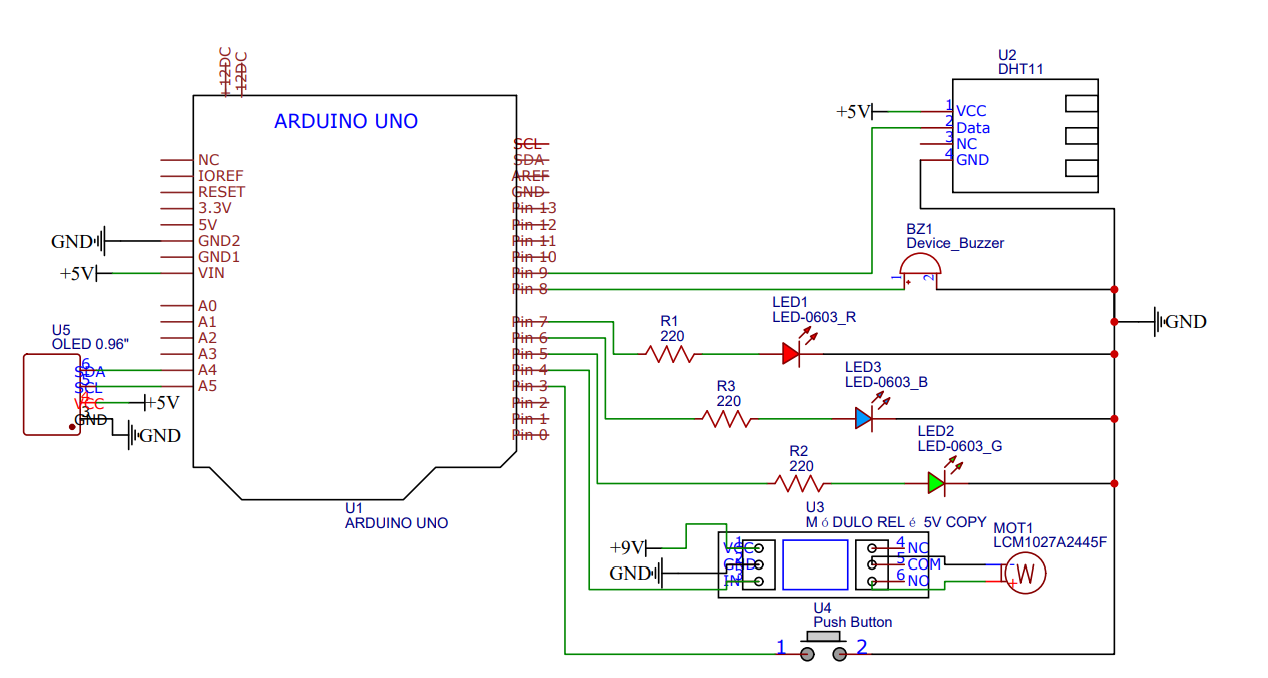
\includegraphics[width=\columnwidth]{images/Imagen_1R3.png}
                  \caption{Esquemático de Conexión Reto 3}
                  \label{fig:Imagen_1R3}
                  \end{figure}
                
            \end{itemize}
    
    \item Código Documentado

    El código propuesto documentado se encuentra registrado a continuación:
    \begin{lstlisting}[caption={Sistema de Riego Automatico con DHT11 y OLED}, label={lst:riego-automatico}]
#include <DHT.h>
#include <Adafruit_GFX.h>
#include <Adafruit_SSD1306.h>
// --- Definicion de pines ---
const int PIN_SENSOR_HUMEDAD = 2;
const int PIN_RELE           = 4;
const int PIN_LED_VERDE      = 5;
const int PIN_LED_AZUL       = 6;
const int PIN_LED_ROJO       = 7;
const int PIN_BUZZER         = 8;
const int PIN_BOTON_MANUAL   = 3;
// --- Configuracion DHT11 ---
#define DHTTYPE DHT11
DHT dht(PIN_SENSOR_HUMEDAD, DHTTYPE);
// --- Configuracion OLED ---
#define SCREEN_WIDTH 128
#define SCREEN_HEIGHT 64
#define OLED_RESET    -1
Adafruit_SSD1306 oled(SCREEN_WIDTH,
                      SCREEN_HEIGHT,
                      &Wire,
                      OLED_RESET);
// --- Umbrales de humedad ---
const int UMBRAL_SECO   = 30;
const int UMBRAL_HUMEDO = 70;
const int UMBRAL_ALARMA = 20;
const int HISTERESIS    = 5;
// --- Temporizacion ---
const long INTERVALO_LECTURA = 2000;
const long TIEMPO_MIN_RIEGO  = 5000;
// --- Enumeracion de estados ---
enum EstadoRiego
{ IDLE, REGANDO, ALARMA };
EstadoRiego estadoRiego = IDLE;
// --- Variables de control ---
float         humedadActual       = 0.0;
bool          bombaActiva         = false;
unsigned long tiempoUltimaLectura = 0;
unsigned long tiempoInicioRiego   = 0;
unsigned long tiempoBuzzer        = 0;
bool          estadoBuzzer        = false;
float leerHumedad() {
  float h = dht.readHumidity();
  if (isnan(h)) {
    Serial.println("Error DHT11");
    oled.clearDisplay();
    oled.setCursor(0, 0);
    oled.println("Error sensor");
    oled.println("DHT11 fallo");
    oled.display();
    return -1.0;
  }
  return h;
}
void activarBomba() {
  if (!bombaActiva) {
    digitalWrite(PIN_RELE, LOW);
    bombaActiva       = true;
    tiempoInicioRiego = millis();
    Serial.println("BOMBA: ACTIVADA");
  }
}
void desactivarBomba() {
  if (bombaActiva) {
    digitalWrite(PIN_RELE, HIGH);
    bombaActiva = false;
    Serial.println("BOMBA: DESACTIVADA");
  }
}
void evaluarEstadoRiego() {
  bool tiempoMinCumplido =
    (millis() - tiempoInicioRiego)
    >= TIEMPO_MIN_RIEGO;
  switch (estadoRiego) {
    case IDLE:
      if (humedadActual < UMBRAL_ALARMA){
        estadoRiego = ALARMA;
        activarBomba();
      } else if (humedadActual
                 <= UMBRAL_SECO) {
        estadoRiego = REGANDO;
        activarBomba();
      }
      break;
    case REGANDO:
      if (tiempoMinCumplido &&
          humedadActual >=
          UMBRAL_HUMEDO) {
        estadoRiego = IDLE;
        desactivarBomba();
      }
      break;
    case ALARMA:
      activarBomba();
      if (humedadActual >=
         (UMBRAL_SECO + HISTERESIS)) {
        estadoRiego = IDLE;
        desactivarBomba();
      }
      break;
  }
}
void actualizarIndicadores() {
  digitalWrite(PIN_LED_VERDE,
               estadoRiego == IDLE);
  digitalWrite(PIN_LED_AZUL,
               estadoRiego == REGANDO);
  digitalWrite(PIN_LED_ROJO,
               estadoRiego == ALARMA);
}
void gestionarBuzzerAlarma() {
  if (estadoRiego != ALARMA) {
    noTone(PIN_BUZZER);
    return;
  }
  if ((millis() - tiempoBuzzer) >= 500){
    tiempoBuzzer = millis();
    estadoBuzzer = !estadoBuzzer;
    if (estadoBuzzer)
      tone(PIN_BUZZER, 880, 250);
    else
      noTone(PIN_BUZZER);
  }
}
void verificarBotonManual() {
  if (digitalRead(PIN_BOTON_MANUAL)
      == LOW) {
    delay(50);
    if (digitalRead(PIN_BOTON_MANUAL)
        == LOW) {
      desactivarBomba();
      estadoRiego = IDLE;
      Serial.println(
        "OVERRIDE: Riego detenido");
    }
  }
}
void mostrarEnOLED() {
  oled.clearDisplay();
  oled.setTextSize(1);
  oled.setTextColor(SSD1306_WHITE);
  oled.setCursor(0, 0);
  oled.println("Sistema de Riego");
  oled.drawLine(0, 10, 127, 10,
                SSD1306_WHITE);
  oled.setTextSize(2);
  oled.setCursor(0, 16);
  oled.print("Hum: ");
  oled.print((int)humedadActual);
  oled.println("%");
  oled.setTextSize(1);
  oled.setCursor(0, 40);
  oled.print("Estado: ");
  switch (estadoRiego) {
    case IDLE:
      oled.println("OPTIMO");   break;
    case REGANDO:
      oled.println("REGANDO");  break;
    case ALARMA:
      oled.println("ALARMA!");  break;
  }
  oled.setCursor(0, 52);
  oled.print("Bomba: ");
  oled.println(bombaActiva ?
  "ON":"OFF");
  oled.display();
}
void setup() {
  Serial.begin(9600);
  dht.begin();
  pinMode(PIN_RELE,         OUTPUT);
  pinMode(PIN_LED_VERDE,    OUTPUT);
  pinMode(PIN_LED_AZUL,     OUTPUT);
  pinMode(PIN_LED_ROJO,     OUTPUT);
  pinMode(PIN_BUZZER,       OUTPUT);
  pinMode(PIN_BOTON_MANUAL,
  INPUT_PULLUP);
  digitalWrite(PIN_RELE, HIGH);
  oled.begin(SSD1306_SWITCHCAPVCC,
             0x3C);
  oled.clearDisplay();
  oled.setTextSize(1);
  oled.setTextColor(SSD1306_WHITE);
  oled.setCursor(20, 20);
  oled.println("Sistema Riego");
  oled.setCursor(25, 35);
  oled.println("Iniciando...");
  oled.display();
  delay(2000);
  oled.clearDisplay();
  Serial.println(
    "Sistema de Riego - Listo");
}
void loop() {
  unsigned long ahora = millis();
  if (ahora - tiempoUltimaLectura
      >= INTERVALO_LECTURA) {
    tiempoUltimaLectura = ahora;
    humedadActual = leerHumedad();
    if (humedadActual < 0) return;
    evaluarEstadoRiego();
    actualizarIndicadores();
    mostrarEnOLED();
    Serial.print("Humedad: ");
    Serial.print(humedadActual);
    Serial.print("% | Estado: ");
    Serial.println(estadoRiego);
  }
  gestionarBuzzerAlarma();
  verificarBotonManual();
}
\end{lstlisting}
\end{itemize}
        